\documentclass[letter,twoside,11pt]{article}

\usepackage[spanish,es-nodecimaldot]{babel}
\usepackage[utf8]{inputenc}

\usepackage{lmodern}
\usepackage[T1]{fontenc}
\usepackage{textcomp}

\usepackage{framed}
\usepackage[svgnames]{xcolor}
\colorlet{shadecolor}{Gainsboro!50}

\usepackage[labelfont=bf]{caption}
\usepackage{graphicx}
\usepackage{pstricks}

\usepackage{anysize}
\marginsize{3cm}{2cm}{2cm}{3cm}

\usepackage{siunitx}
\usepackage{amsmath}
\usepackage{array}
\usepackage{csquotes}

\usepackage{fancyhdr}
\usepackage{lastpage}
\pagestyle{fancy}
\fancyhf{}
\fancyhead[LE,RO]{Laboratorio de Electrónica Analógica I}
\fancyfoot[CO,CE]{\thepage\ de \pageref{LastPage}}

\special{papersize=215.9mm,279.4mm}

\usepackage[
    pdfauthor={Carlos Eduardo Caballero Burgoa},%
    pdftitle={Laboratorio de Electrónica Analógica I},%
    pdfsubject={Fuentes de alimentación DC, generador de funciones y osciloscopio},%
    colorlinks,%
    citecolor=black,%
    filecolor=black,%
    linkcolor=black,%
    urlcolor=black,
    breaklinks]{hyperref}
\usepackage{breakurl}

\newcommand{\blankpage}{
\newpage
\thispagestyle{empty}
\mbox{}
\newpage
}

\renewcommand{\arraystretch}{1.2}

\begin{document}

\begin{titlepage}
    \begin{center}
        {\Large UNIVERSIDAD MAYOR DE SAN SIMÓN}\\
        \vspace*{0.15cm}
        {\large FACULTAD DE CIENCIAS Y TECNOLOGÍA}\\
        \vspace*{0.10cm}
        DEPARTAMENTO DE ELÉCTRICA-ELECTRÓNICA\\
        \vspace*{3.0cm}
        {\Large \textbf{LABORATORIO DE ELECTRÓNICA ANALÓGICA I}}\\
        \vspace*{0.3cm}
        {\Large \textbf{REPORTE No. 1}}\\
        \vspace*{3.5cm}
        {\Large \textbf{FUENTES DE ALIMENTACIÓN DC, GENERADOR DE \\ FUNCIONES Y EL OSCILOSCOPIO}}\\
    \end{center}

    \vspace*{5.8cm}
    \leftskip=7.95cm
    \noindent
    \textbf{Estudiante:}\\
    Caballero Burgoa, Carlos Eduardo.\\
    \newline
    \textbf{Carrera:}\\
    Ing. Electromecánica.\\
    \newline
    \textbf{Docente:}\\
    Ing. Alberto Arispe Santander.\\
    \newline
    \textbf{Grupo:} 1B.\\
    \textbf{Fecha de entrega:} 17 de Septiembre del 2024.\\
\end{titlepage}
\addtocounter{page}{-1}

\blankpage
\addtocounter{page}{-1}

\section{Fuente de alimentación DC}
Las fuentes de alimentación $DC$ son dispositivos que a partir de la tensión de
red son capaces de proporcionar una señal de tensión continua para alimentar al
circuito al que se conecta.

Una fuente de alimentación $AC/DC$ funciona mediante la \textbf{rectificación} y
la \textbf{regulación} de la corriente alterna de entrada para proporcionar una
corriente continua de salida con la tensión y la corriente adecuadas para el
dispositivo que se va a alimentar.

\subsection{Características}

\begin{description}
    \item [Voltaje de salida estable] Deben proporcionar un voltaje de salida
    estable y confiable, independientemente de las fluctuaciones en el voltaje
    de entrada o las cargas conectadas al sistema.
    \item [Regulación de la tensión y la corriente] Suelen incluir circuitos de
    regulación que ajustan la tensión y la corriente de salida para garantizar
    un suministro constante y seguro.
    \item [Eficiencia energético] Las fuentes de alimentación modernas están
    diseñadas para ser altamente eficientes, minimizando las perdidas de energía
    durante la conversión de corriente alterna a corriente continua.
    \item [Protecciones de seguridad] Suelen incluir protecciones de seguridad
    integradas, como protección contra sobre-tensión, sobre-corriente y
    cortocircuitos, para la protección tanto de la fuente de alimentación como
    los dispositivos conectados de daños potenciales.
    \item [Compatibilidad internacional] Muchas están diseñadas para ser
    compatibles con diferentes estándares de enchufes y voltajes de entrada.
\end{description}

\subsection{Funcionamiento}
Una fuente de alimentación $AC/DC$ funciona mediante un proceso de conversión de
corriente alterna en corriente continua, que es la forma de energía eléctrica
utilizada por la mayoría de los dispositivos electrónicos.

De esta manera, el primer paso en la conversión es la rectificación; proceso
donde se transforma la corriente alterna de entrada en corriente pulsante de
polaridad única. Esto se logra mediante el uso de diodos rectificadores que
permiten que la corriente fluya en una sola dirección. Dependiendo del diseño de
la fuente de alimentación, este proceso puede ser de media onda o de onda
completa.

Después de la rectificación, la corriente pulsante aún contiene componentes de
alta frecuencia no deseados. Para suavizar la corriente y eliminar estas
fluctuaciones no deseadas se utiliza un filtro, generalmente compuesto por
condensadores, que suaviza la salida para producir una corriente más cercana a
una señal continua.

Una vez que se ha rectificado y filtrado la corriente, se regula para asegurar
que el voltaje de salida sea estable y se mantenga dentro de los límites
deseados, independientemente de las fluctuaciones en el voltaje de entrada o la
carga conectada. Esto se logra mediante el uso de circuitos de regulación que
ajustan la tensión de salida según sea necesario.

Finalmente, la corriente continua regulada y filtrada se utiliza para alimentar
los dispositivos electrónicos conectados a la fuente de alimentación. Estos
dispositivos operan con corriente continua y utilizan la energía proporcionada
por la fuente de alimentación para su funcionamiento.

\subsection{GPS-3030DD}
La fuente de alimentación hallada en laboratorio consta de las siguientes
funciones:

\begin{figure}[!h]
\centering
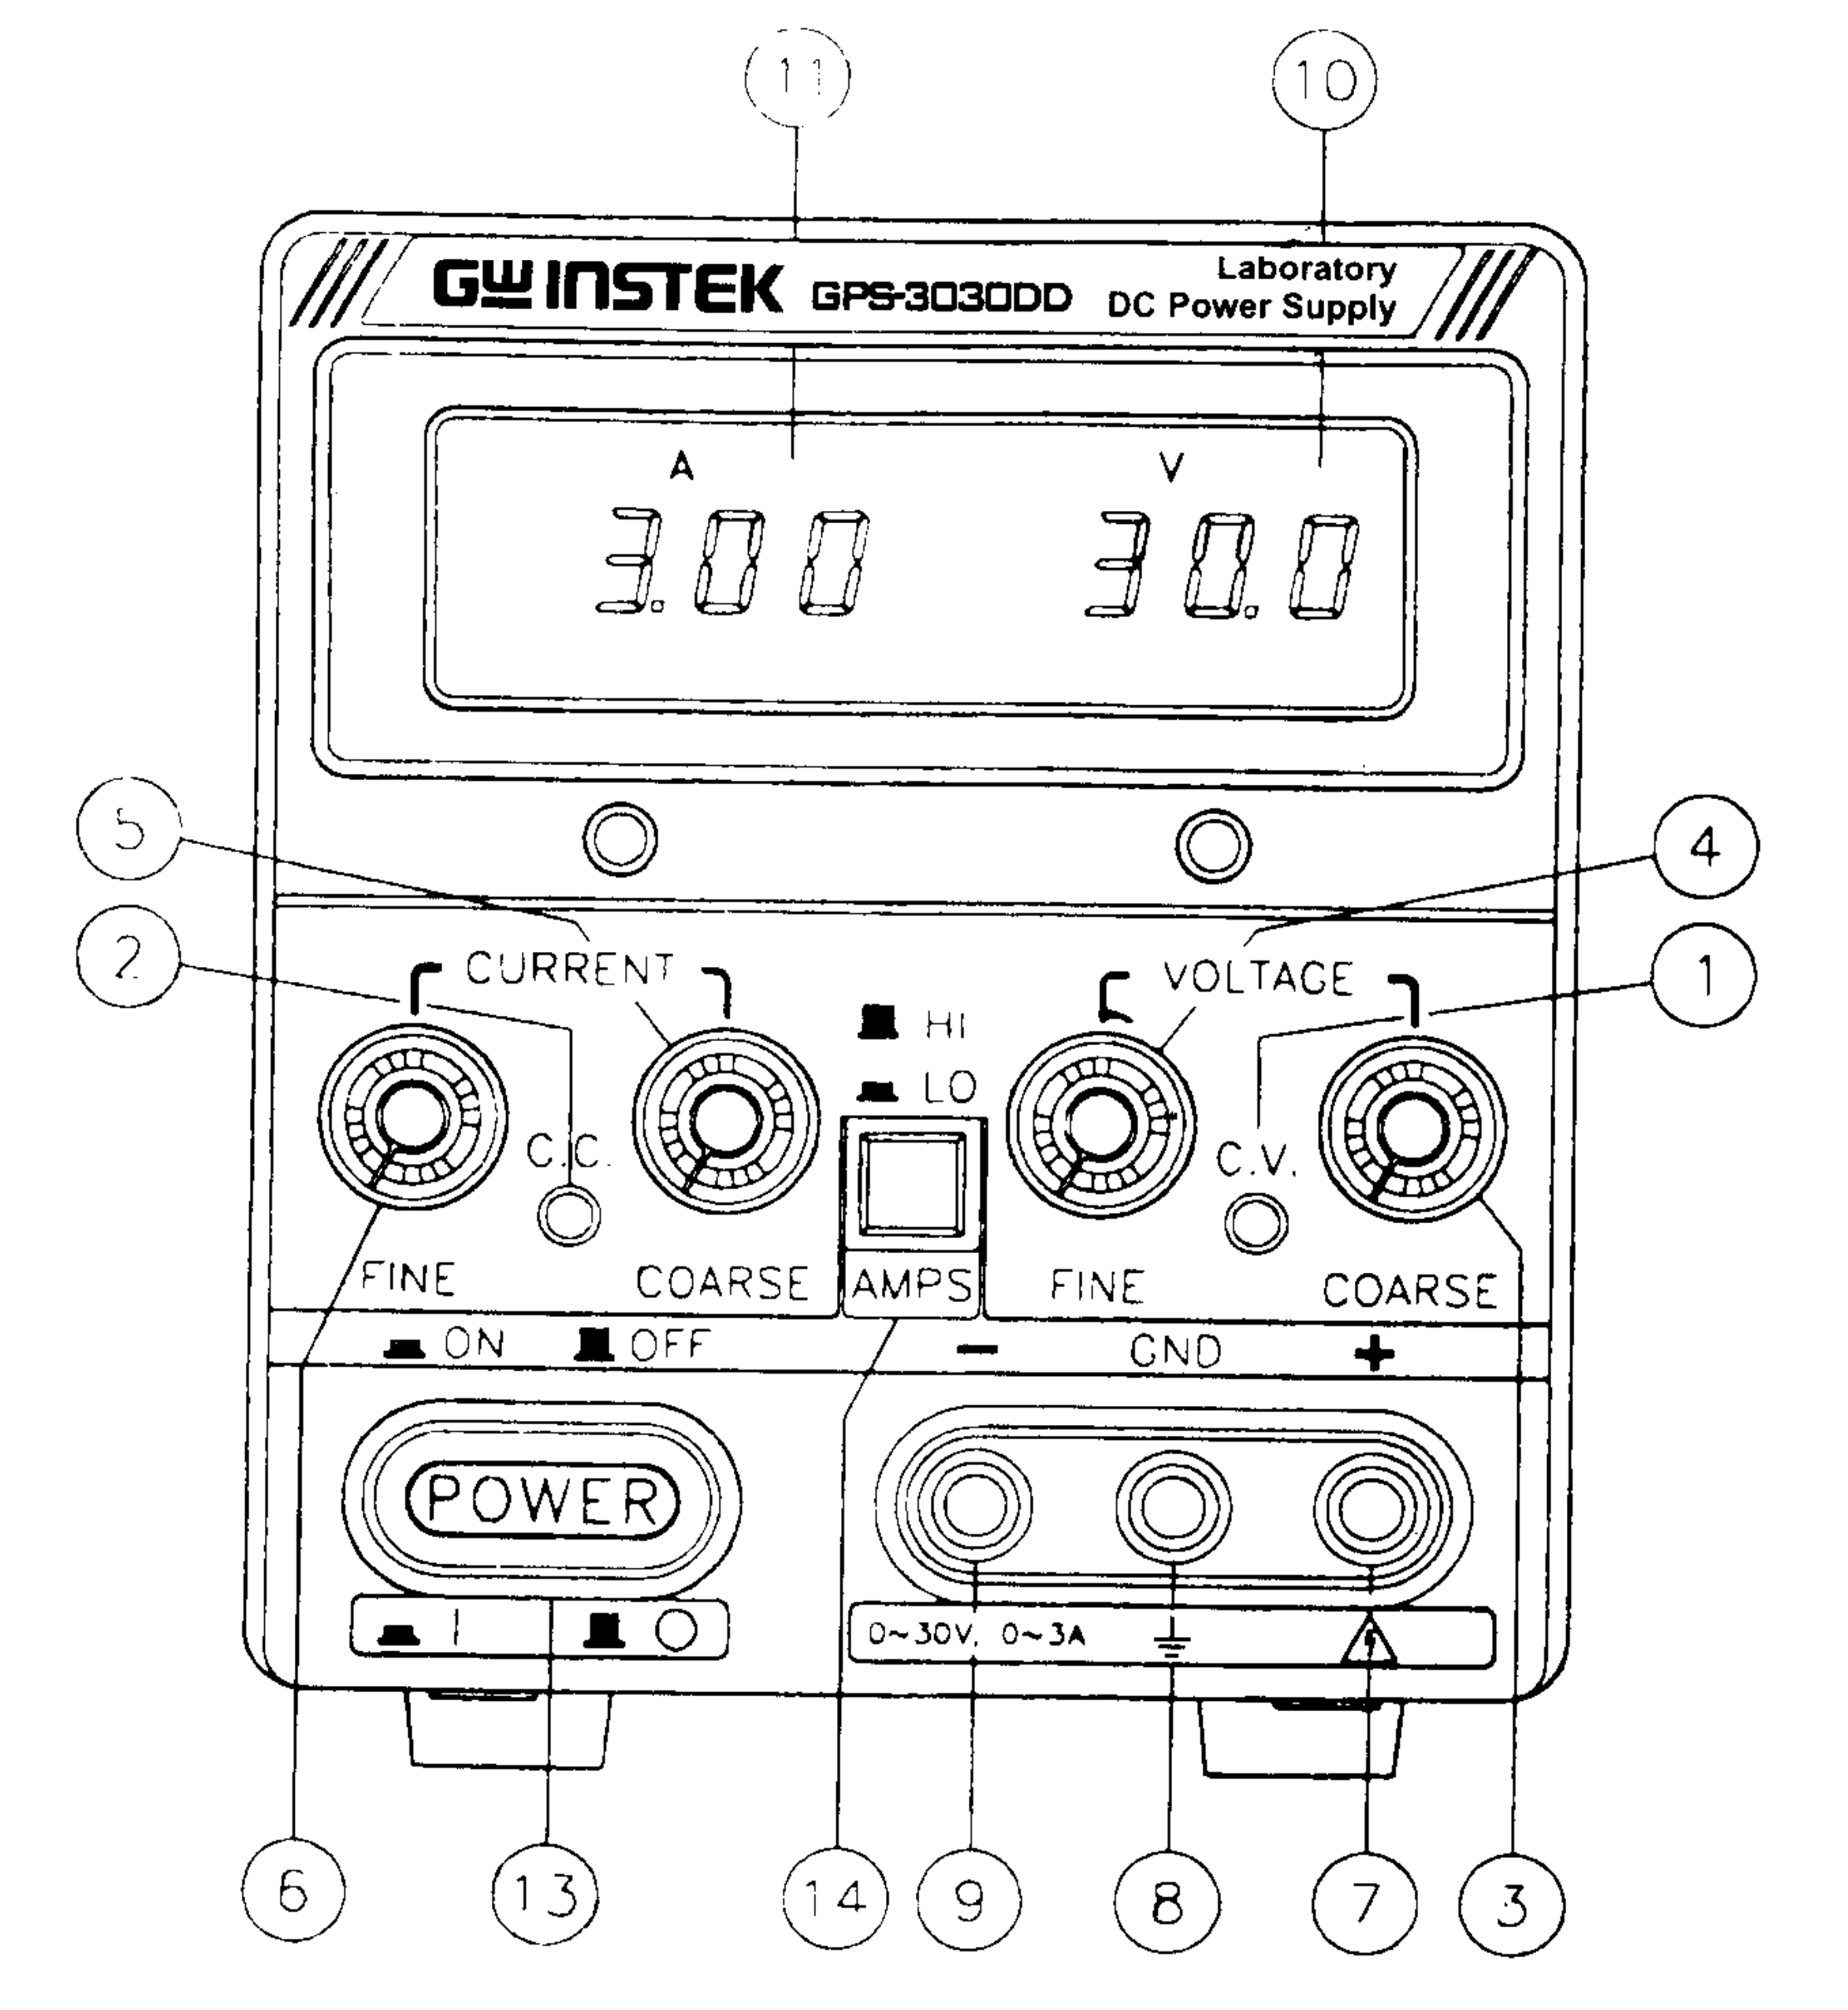
\includegraphics[scale=0.25]{figura1.eps}
\caption{Panel frontal.}
\end{figure}

\begin{enumerate}
    \item Indicador de operación en voltaje constante.
    \item Indicador de operación en corriente constante.
    \item Ajuste grueso del voltaje de salida.
    \item Ajuste fino del voltaje de salida.
    \item Ajuste grueso de la corriente de salida.
    \item Ajuste fino de la corriente de salida.
    \item Polaridad positiva (Rojo).
    \item Tierra y puesta a tierra del chasis (Verde).
    \item Polaridad negativa (Negro).
    \item Indicador del voltaje de salida.
    \item Indicador de la corriente de salida.
        \setcounter{enumi}{12}
    \item Interruptor de encendido/apagado.
    \item Indicador de rango alto o bajo.
\end{enumerate}

\section{Generador de funciones}
Un generador de funciones es un dispositivo electrónico que permite al usuario
generar diferentes tipos de onda predefinidas tales como: senoidal, cuadrada,
triangular, pulso o ruido eléctrico; con características ajustables y de alta
precisión tales como: la frecuencia y la amplitud.

La función principal de un generador de funciones es la de producir señales
periódicas o no periódicas, aplicándose normalmente en el diseño, prueba y
reparación de dispositivos electrónicos; aunque también puede tener usos
artísticos y ser empleado en la medicina.

\subsection{Usos}
En cuanto a los usos y funciones más comunes del generador de funciones, se
diferencian:

\begin{description}
    \item [Creación de señales] Creadas desde cero para simular, estimular y
    probar distintos circuitos y dispositivos.
    \item [Replicación de señales] ya sea una anomalía, un error o una señal
    adquirida por un osciloscopio, se puede replicar utilizando un generador de
    funciones en un laboratorio para variar sus parámetros y analizarla en un
    ambiente controlado.
    \item [Generación de señales] Señales ideales o funciones ya conocidas para
    utilizarlas como referencia o como señal de entrada para pruebas.
\end{description}

\subsection{SFG-1013}
El generador de señales hallado en laboratorio consta de las siguientes
funciones:

\begin{figure}[!h]
\centering
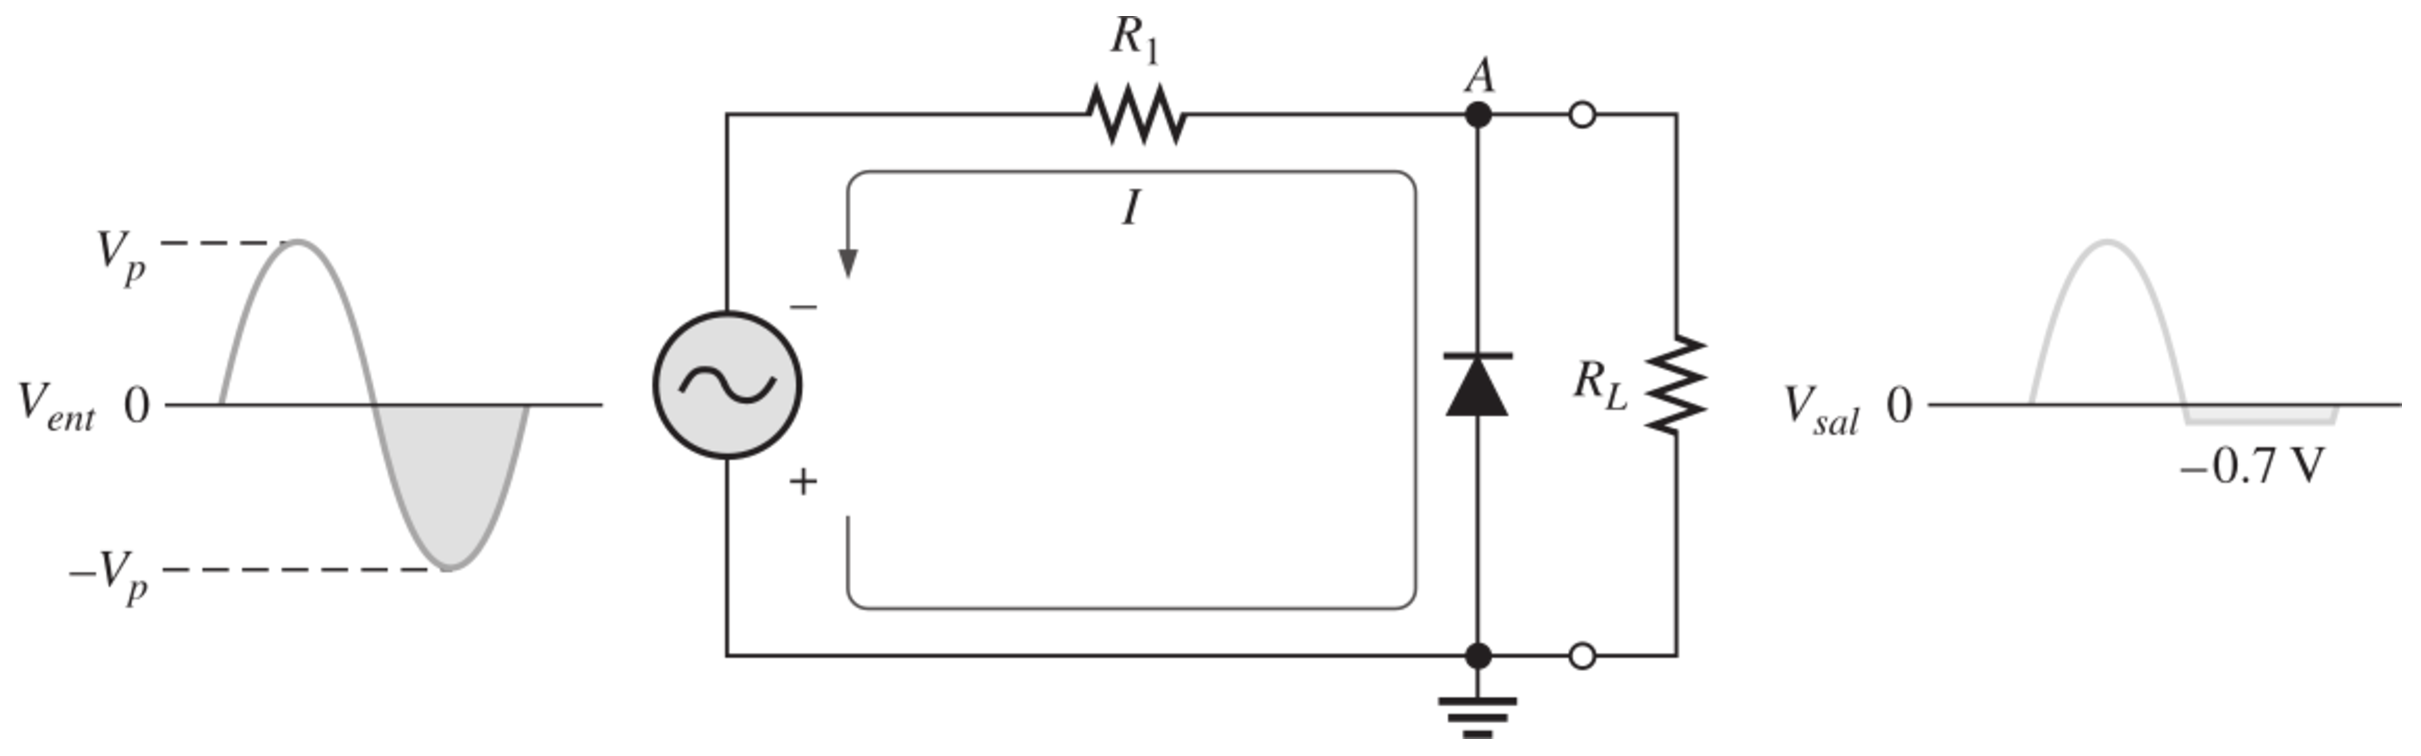
\includegraphics[scale=0.40]{figura2.eps}
\caption{Panel frontal.}
\end{figure}

\begin{description}
    \item [Main Display] Pantalla principal.
    \item [Entry keys] Teclas de entrada.
    \item [Shift keys] Teclas de cambio.
    \item [Output On/Off key] Tecla de encendido/apagado de salida.
    \item [Power Switch] Interruptor de encendido.
    \item [Frecuency Adjustment Knob] Perilla de ajuste de frecuencia.
    \item [Duty Control] Ajuste de forma en función cuadrada.
    \item [Offset Control] Ajuste de compensación.
    \item [Amplitud Control] Ajuste de amplitud.
    \item [TTL Output] Salida TTL.
    \item [Main Output] Salida principal.
\end{description}

\section{Osciloscopio}
Un osciloscopio es un instrumento de medición que permite visualizar señales
eléctricas en una pantalla, a fin de analizar su comportamiento. Es uno de los
equipos más útiles del laboratorio de electrónica. Las señales se muestran en
gráficos donde un haz de electrones pasa a través de un eje de coordenadas en
una pantalla de fósforo. La amplitud se muestra en el eje vertical y el tiempo
en el eje horizontal. La imagen resultante de la medición se conoce como
oscilograma.

\subsection{Características}
El osciloscopio mide lo siguiente:

\begin{itemize}
    \item Valores de tiempo y voltaje de una señal.
    \item Frecuencia de una señal oscilante.
    \item Frecuencia con la que se produce una parte especifica de la señal en
        relación con otras.
    \item Si un componente que funciona mal esta distorsionando o no la señal.
    \item Que tanto de una señal es de corriente continua o alterna.
    \item La porción de la señal que es ruido.
    \item Si el ruido cambia con el tiempo.
\end{itemize}

\subsection{GOS-630FC}
El osciloscopio utilizado en laboratorio consta de las siguientes funciones:

\begin{figure}[!h]
\centering
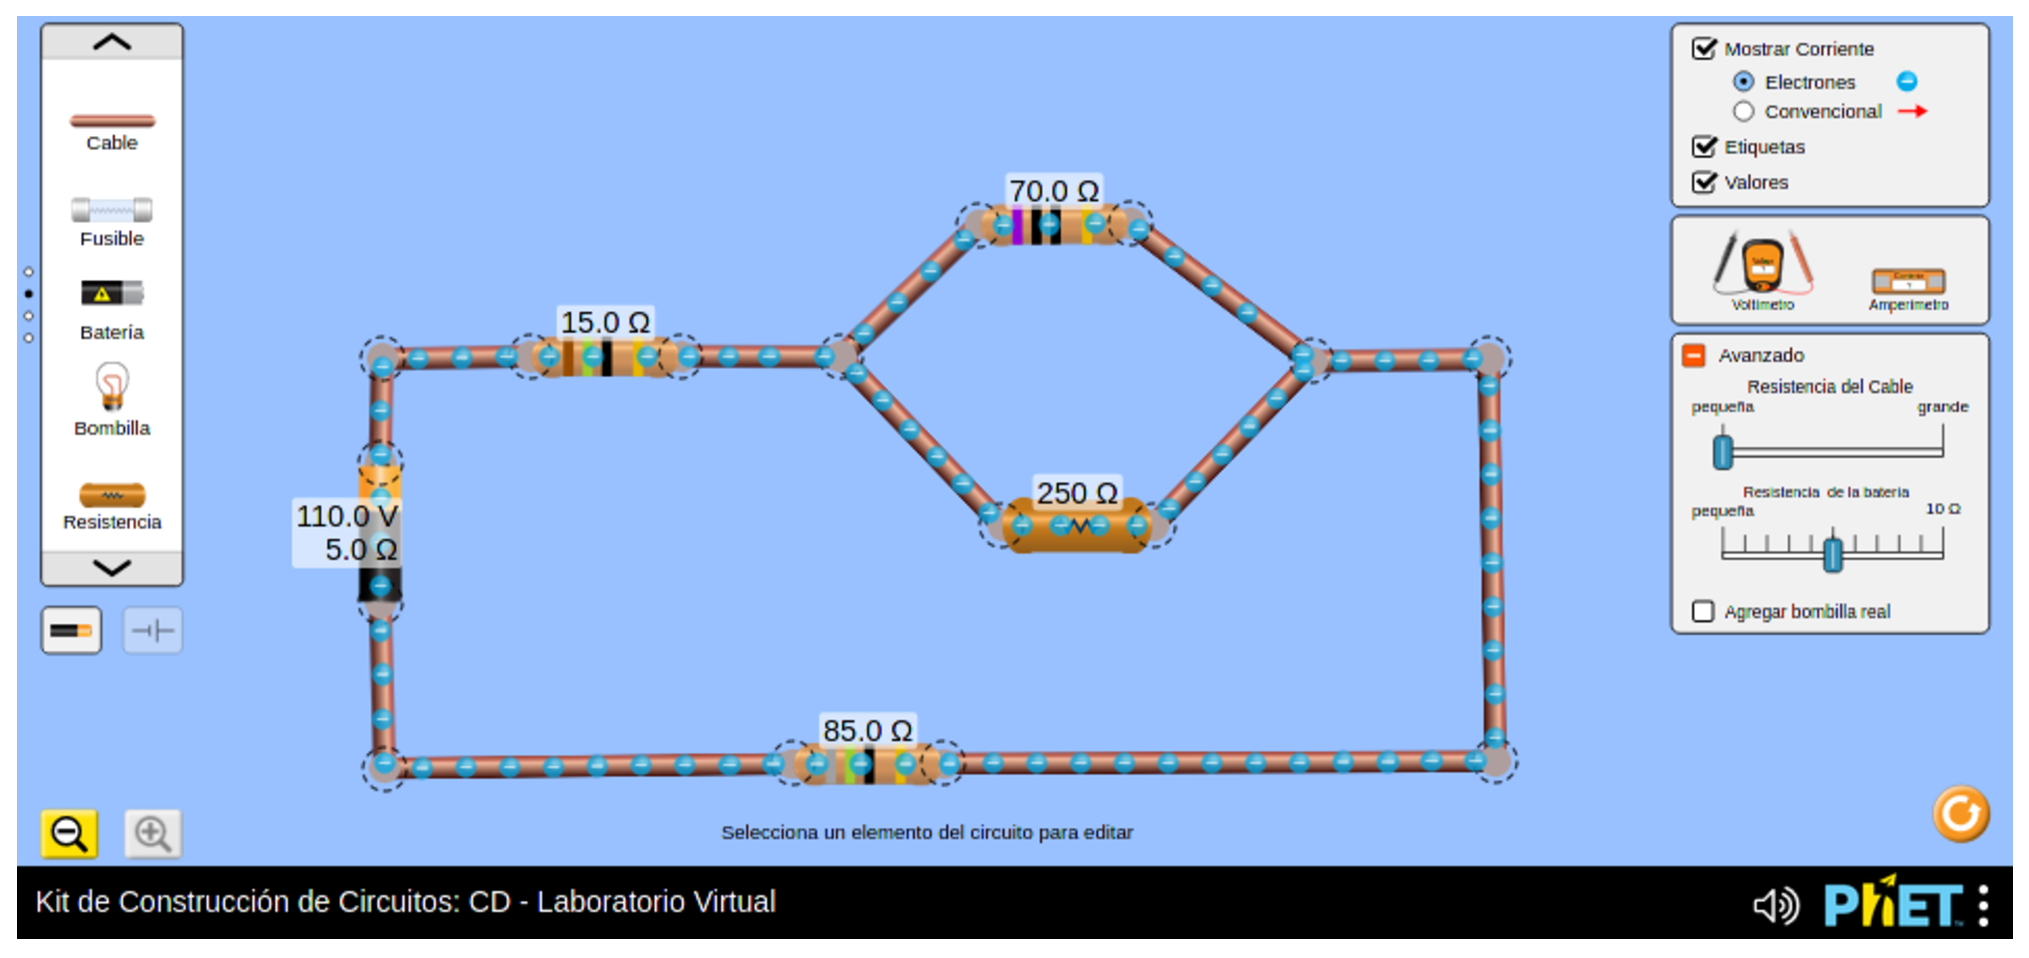
\includegraphics[scale=1.3]{figura3.eps}
\caption{Panel frontal.}
\end{figure}

\begin{description}
    \item [Main Display] Presenta la forma de onda de las señales de entrada.
    \item [Display Controls] Controles de encendido, configuración de pantalla
    y la salida de compensación de la sonda.
    \item [LCD Display] Presenta la escala vertical, escala horizontal, modo de
    visualización X-Y, y la frecuencia de la forma de onda.
    \item [Horizontal Controls] Controles para la escala horizontal, posición
    horizontal, longitud de barrido, y magnificador.
    \item [Vertical Controls] Controles para la escala vertical, posición
    vertical, modo de presentación, inversión del canal secundario y modo de
    visualización alternativo.
    \item [Trigger Controls] Controles del modo de disparo, nivel de activación,
    fuente de acoplamiento del disparador, pendiente de activación y modo de
    activación alternativo.
    \item [Input Terminals] Acepta las señales de entrada de canal 1 y canal 2
    y el cable de tierra. Controla el modo de acoplamiento de la señal de
    entrada.
\end{description}

\begin{thebibliography}{99}

\bibitem{FADC} Fuentes de alimentación DC \\
Extraído el 16 de Septiembre del 2024, de: \\
\url{https://isotest.net/productos/fuentes-alimentacion-dc/}.

\bibitem{FAACDC} Fuente de alimentación AC/DC: ¿Qué diferencias presentan? \\
Extraído el 16 de Septiembre del 2024, de: \\
\url{https://distron.es/fuente-de-alimentacion-ac-dc/}.

\bibitem{DCPS} DC Power Supply. User Manual \\
Extraído el 16 de Septiembre del 2024, de: \\
\url{https://www.gwinstek.com/en-global/products/detail/GPS-Series}

\bibitem{GSCA} Generador de señal: Características y aplicaciones \\
Extraído el 16 de Septiembre del 2024, de: \\
\url{https://distron.es/generador-de-senal/}

\bibitem{SFG} Synthesized Function Generator. User Manual \\
Extraído el 16 de Septiembre del 2024, de: \\
\url{https://www.gwinstek.com/en-global/products/detail/SFG-1000}

\bibitem{QEUO} ¿Qué es un osciloscopio? \\
Extraído el 16 de Septiembre del 2024, de: \\
\url{https://www.330ohms.com/blogs/blog/que-es-un-osciloscopio}

\bibitem{PQUO} ¿Para qué se usa un osciloscopio? \\
Extraído el 16 de Septiembre del 2024, de: \\
\url{https://www.tecsaqro.com.mx/blog/osciloscopio/}

\bibitem{DTO} Dual Trace Oscilloscope. User Manual \\
Extraído el 16 de Septiembre del 2024, de: \\
\url{https://www.gwinstek.com/en-IN/products/detail/GOS-630FC}

\end{thebibliography}

\end{document}

